\section{Conventional Methods in Action Recognition}
META: 
Condensed overview and description of conventional Methods in action Recognition using the taxonomy of Aggarwal and Ryoo's fine survey paper.
More detailed description of methods using local-features, since these have become the standard approach in action recognition after Aggarwal and Ryoo's overview.

\begin{figure}[H]
    \centering
    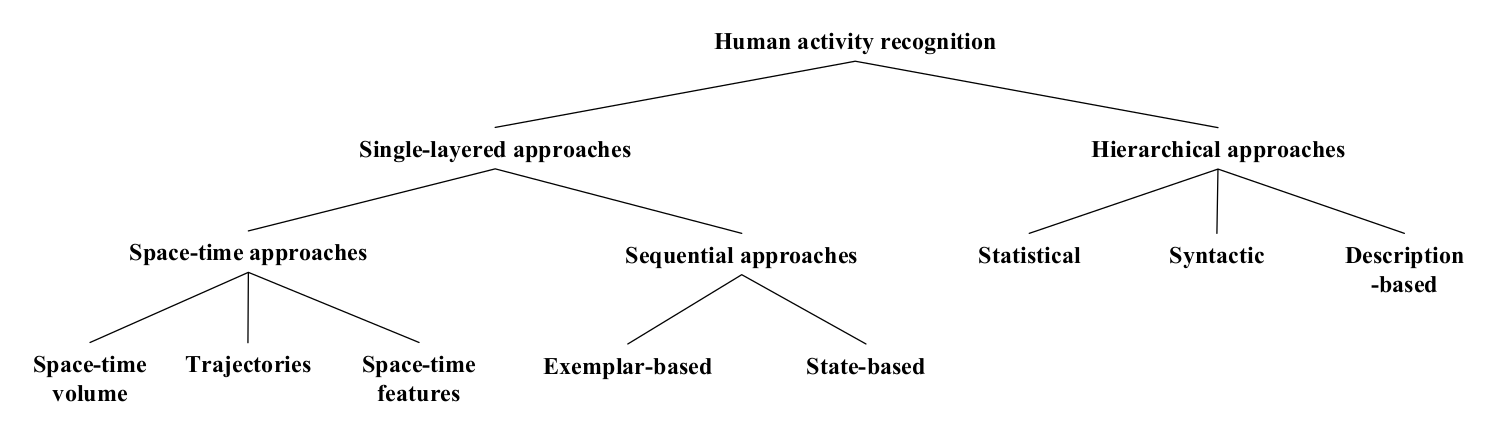
\includegraphics[width=\textwidth]{img_conventional/taxonomy_conventional_methods.png}
    \caption{Approach-based taxonomy for conventional methods in human activity recognition as given by Aggarwal and Ryoo\cite{aggarwal_human_2011}}
    \label{fig:conventional_taxonomy}
\end{figure}

3 Main components in action recognition using local features: Feature Extraction, Representation Building, Classification.

Methods for feature extraction: Interest point detectors or dense sampling.

Space-time interest point detectors: Harris3D\cite{laptev_space-time_2005}, Cuboids\cite{dollar_behavior_2005}, Hessian Detector\cite{willems_efficient_2008}

Descriptors for 3D volumes around previously detected space-time interest points: Histogram of Gradient HOG\cite{dalal_histograms_2005-1}, Histogram of Optical Flow (HOF)\cite{laptev_learning_2008}, 3D Histogram of Gradient (HOG3D)\cite{klaser_spatio-temporal_2008}, Extended SURF (ESURF)\cite{willems_efficient_2008}
